%\documentclass[dvipdfmx,fleqn]{beamer}
\documentclass[dvipdfmx,fleqn,handout]{beamer}
\usepackage{amsmath,amssymb,amsthm}

\mode<presentation>
{
  \usetheme{Lleida}
}

\title{\Large Fictitiouos Play}
\author{\large 小川慶将}
\date{\small 2014.6.28}

\usefonttheme{professionalfonts}

\setbeamercovered{transparent=20}

\setbeamertemplate{navigation symbols}{} 
\setbeamertemplate{footline}[frame number] 



\begin{document}

\sffamily
\gtfamily


\begin{frame}
  \titlepage
  \thispagestyle{empty}
\end{frame}

\setcounter{framenumber}{0}




\begin{frame}
\frametitle{はじめに}
\begin{itemize}\setlength{\parskip}{0.5em}
\item
Fictitious Playとは?
 \begin{itemize}\setlength{\parskip}{0.5em}
 \item
 日本名では仮想ゲームなどと呼ばれる。
 \item
 各プレイヤーがそれぞれの予想のもとで最適反応戦略を選択する動学ゲーム。
 \end{itemize}
\end{itemize}
\end{frame}



\begin{frame}
\frametitle{Ficititious playの説明}
\begin{itemize}\setlength{\parskip}{0.5em}
\item
予想の立て方
各 t 時点において,プレイヤー 0 は 「プレイヤー 1 は,確率 1−x0(t) で行動 0 をとり,確率 x0(t) で行動 1 をとる」 と考え,自分の期待利得が最大になるような行動をとる。
x0(t) を「t 時点における,プレイヤー 0 の,プレイヤー 1 の行動に関する信念 (belief)」と呼ぶことにする。(ゼミ課題文より)
\item
予想形成 \pause

$x_0(t)$ は
\[
x_0(t+1)
= x_0(t) + \frac{1}{t+2} (a_1(t) - x_0(t))
\]
と再帰的に書くことができる. \pause
\end{itemize}
\end{frame}


\begin{frame}[fragile]% verbatim 環境を使えるように
\frametitle{工夫した点}
\begin{itemize}\setlength{\parskip}{0.5em}
\item
switchを使用
\begin{verbatim}

その場で入力を要求させるcase0
MachinPenniesをcase1
Coordination Gameをcase2
Prisoner's Dilemmaをcase3

\end{verbatim}
\end{itemize}
\end{frame}


\begin{frame}[fragile]% verbatim 環境を使えるように
\frametitle{コードの説明とか}
\begin{itemize}\setlength{\parskip}{0.5em}
\item
コードの表示の例
\begin{verbatim}
if NUM == 0:
    print '2×2の利得表をひとつずつ記入してください'
    pr_0_00 = float(raw_input('プレイヤー0左上:'))
    pr_0_01 = float(raw_input('プレイヤー0右上:'))
    pr_0_10 = float(raw_input('プレイヤー0左下:'))
    pr_0_11 = float(raw_input('プレイヤー0右下:'))
    pr_1_00 = float(raw_input('プレイヤー1左上:'))
    pr_1_01 = float(raw_input('プレイヤー1右上:'))
    pr_1_10 = float(raw_input('プレイヤー1左下:'))
    pr_1_11 = float(raw_input('プレイヤー1右下:'))
    titlename = raw_input('タイトル名:')
    #player
    p0 = np.array([[pr_0_00,pr_0_01],[pr_0_10,pr_0_11]])
    p1 = np.array([[pr_1_00,pr_1_10],[pr_1_01,pr_1_11]])
\end{verbatim}
\end{itemize}
\end{frame}

\begin{frame}[fragile]% verbatim 環境を使えるように
\frametitle{コードの説明とか}
\begin{itemize}\setlength{\parskip}{0.5em}
\item
コードの表示の例
\begin{verbatim}
#Maching Pennies
if NUM == 1:
    titlename = 'Matching Pennies'
    p0 = np.array([[1,-1],[-1,1]])
    p1 = np.array([[-1,1],[1,-1]])
#Coordination Game
if NUM == 2:
    titlename = 'Coordination Game'
    p0 = np.array([[4,0],[3,2]])
    p1 = np.array([[4,0],[3,2]])
#Prisoner's Dilemma
if NUM == 3:
    titlename = 'Prisoners Dilemma'
    p0 = np.array([[-5,0],[-10,-3]])
    p1 = np.array([[-5,0],[-10,-3]])
\end{verbatim}
\end{itemize}
\end{frame}

\begin{frame}
\frametitle{図}
\begin{figure}
 \centering
 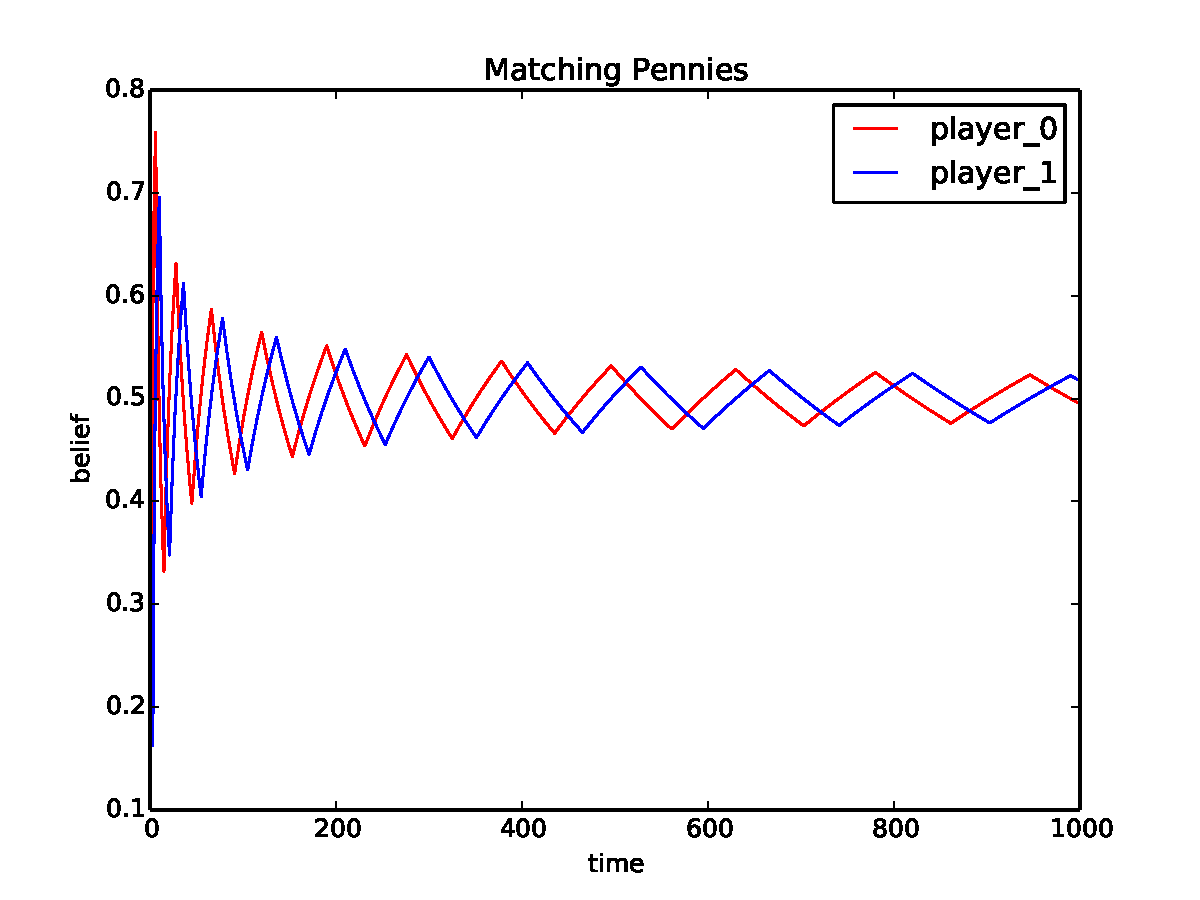
\includegraphics[width=80mm]{matchingpennies_plot.pdf}
 \caption{図の表示}
 \label{fig:matchingpennies_plot}
\end{figure}
\end{frame}



\begin{frame}
\frametitle{まとめ}
\begin{itemize}\setlength{\parskip}{0.5em}
\item
まとめ

-2×2のFictitiousPlayがプログラムを動かすことでナッシュ均衡がすぐに見つかる。

-囚人のジレンマは信念とか全く関係ないですけど動かしてみたらちゃんとみんな自白しました。
\item
よくわかっていない点とか

-スライドの作り方へたくそすぎましたすいません。

-次はもっときれいなの作ります

\item
今後の課題とか

-3×3ゲームでのプログラムも作りたいです。
\end{itemize}
\end{frame}



\end{document}